\section{Transaction Validation}\label{transaction-validation}

The transaction validation process is similar to Bitcoin's unspent transaction output (UTXO) model. An unspent transaction output is the output of a transaction that a user receives and is able to spend in the future. Thus, the validating node must check all previously made transactions of the sender address in order to verify a transaction. The smallest unit of the underlying currency is also called IOTA. All IOTA are minted in the genesis transaction and therefore, every IOTA can be traced back to genesis block. 

Transactions cannot be seen as valid as soon as one approver has referenced it. Thus, a new parameter is introduced called confirmation confidence. The confirmation confidence for a transaction $X$ can be calculated in the following way.

\begin{enumerate}
    \item The tip selection algorithm is run 100 times.
    \item The number of tips that approve transaction $X$ is counted.
    \item Every tip is weighted by the likelihood that it will be accepted in the future.
    \item The confirmation confidence of transaction $X$ is the fraction of approving transactions.
\end{enumerate}

It is assumed that transactions are issued by a large number of independent entities, so the process of incoming transactions can be modeled Poisson point process \cite{the-tangle}. $\lambda$ denotes the rate of the Poisson process and it is assumed that it remains constant in time. At some point in time, every new transaction will approve transaction $X$ since all tips include a path to transaction $X$. Thus, after the adoption period, the cumulative weight will grow linearly with $\lambda * w$ where $w$ is the average weight of a transaction.

\begin{figure}[H]
    \centering
    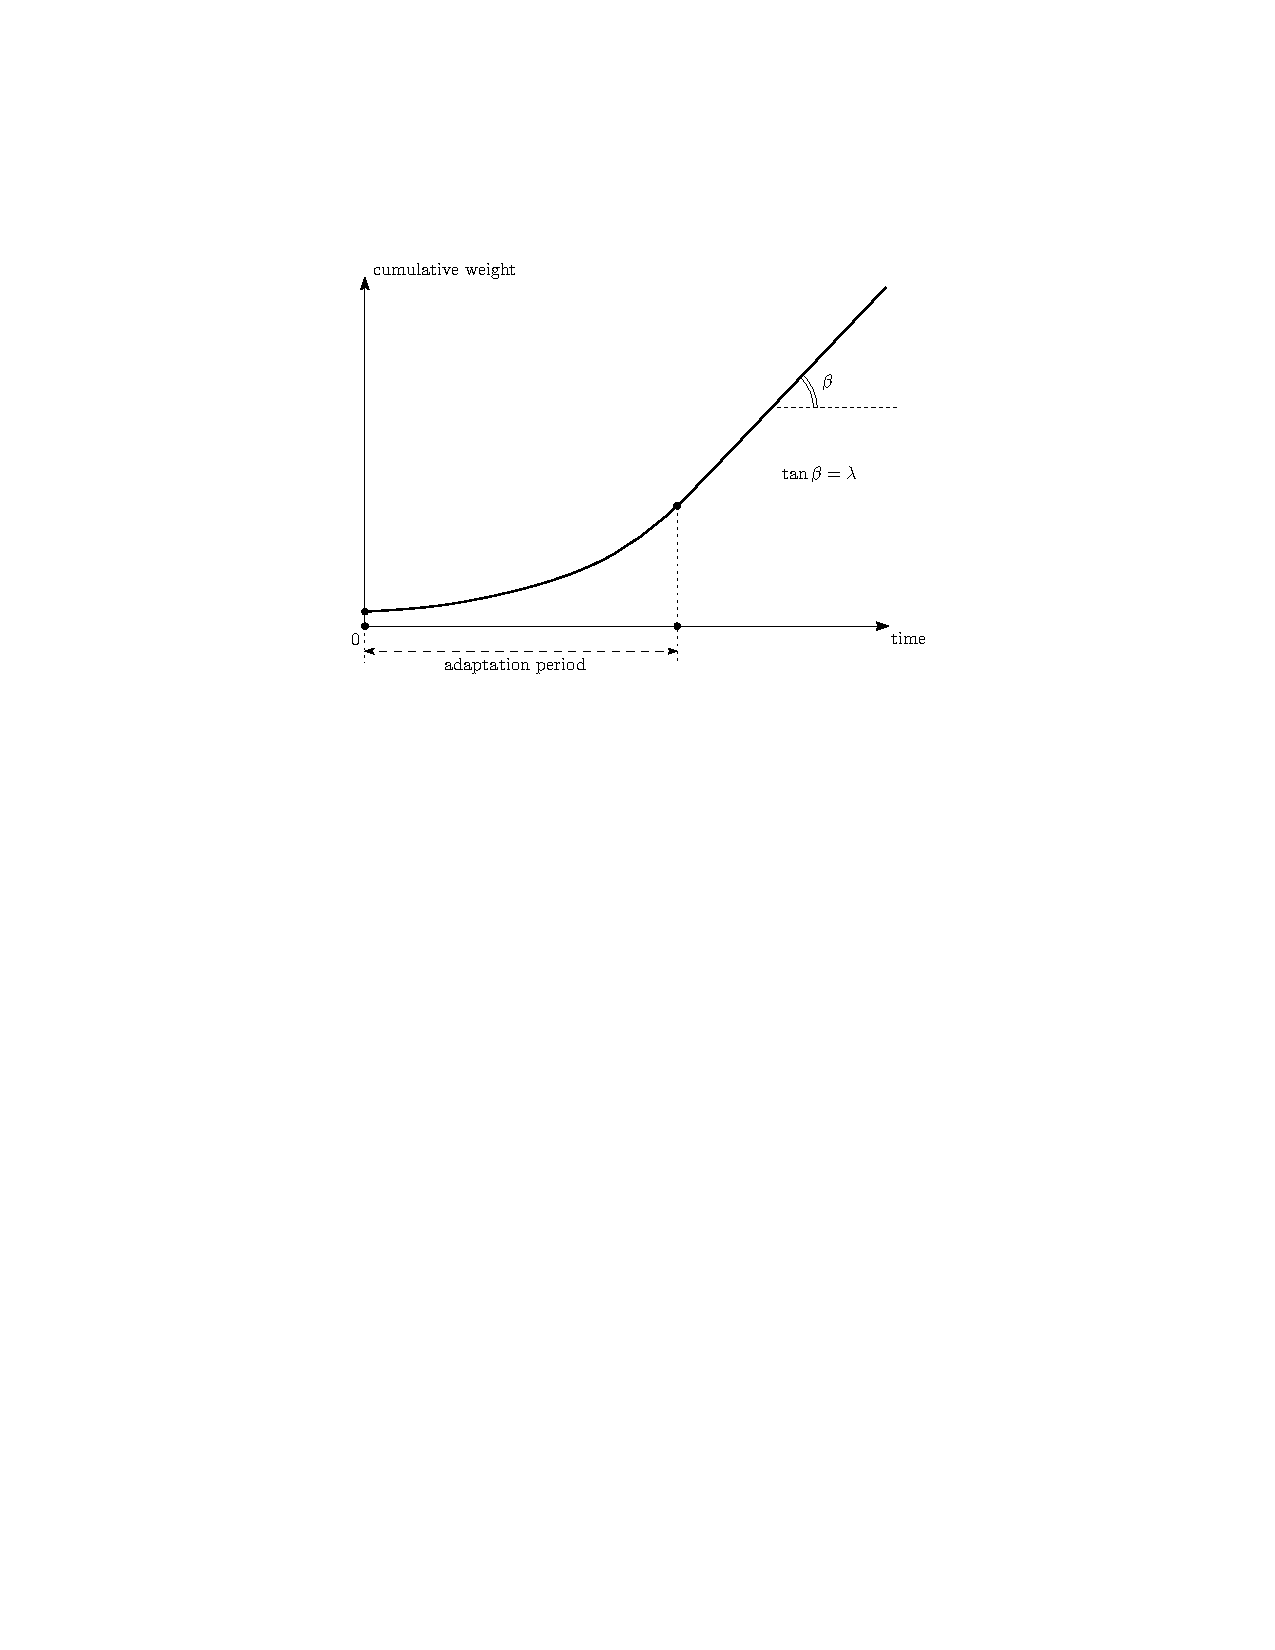
\includegraphics[width=8cm]{images/confirmation-confidence.pdf}
    \caption{Confirmation Confidence and Cumulative Weight Growth \cite{the-tangle}}
    \label{fig:confirmation-confidence}
\end{figure}

In Figure \ref{fig:confirmation-confidence-tangle}, transactions with confirmation confidence of more than 0.95 have a thick border. Almost any new honest transaction that is added to this tangle will confirm these transactions (except lazy nodes with lazy tip selection). In the shown example, transaction 9 confirms all the red transactions and is confirmed by the blue transactions. There are four tips in the shown simulation - 6, 10, 11 and 12. The confirmation confidence of transaction 9 is 0.94 due to the fact that transactions 10, 11 and 12 have more importance than 6.
Transaction 4 has confirmation confidence of 1 since all tips have a path to transaction 4 and therefore, there is no transaction in the network that does not confirm this transaction.

\begin{figure}[H]
    \centering
    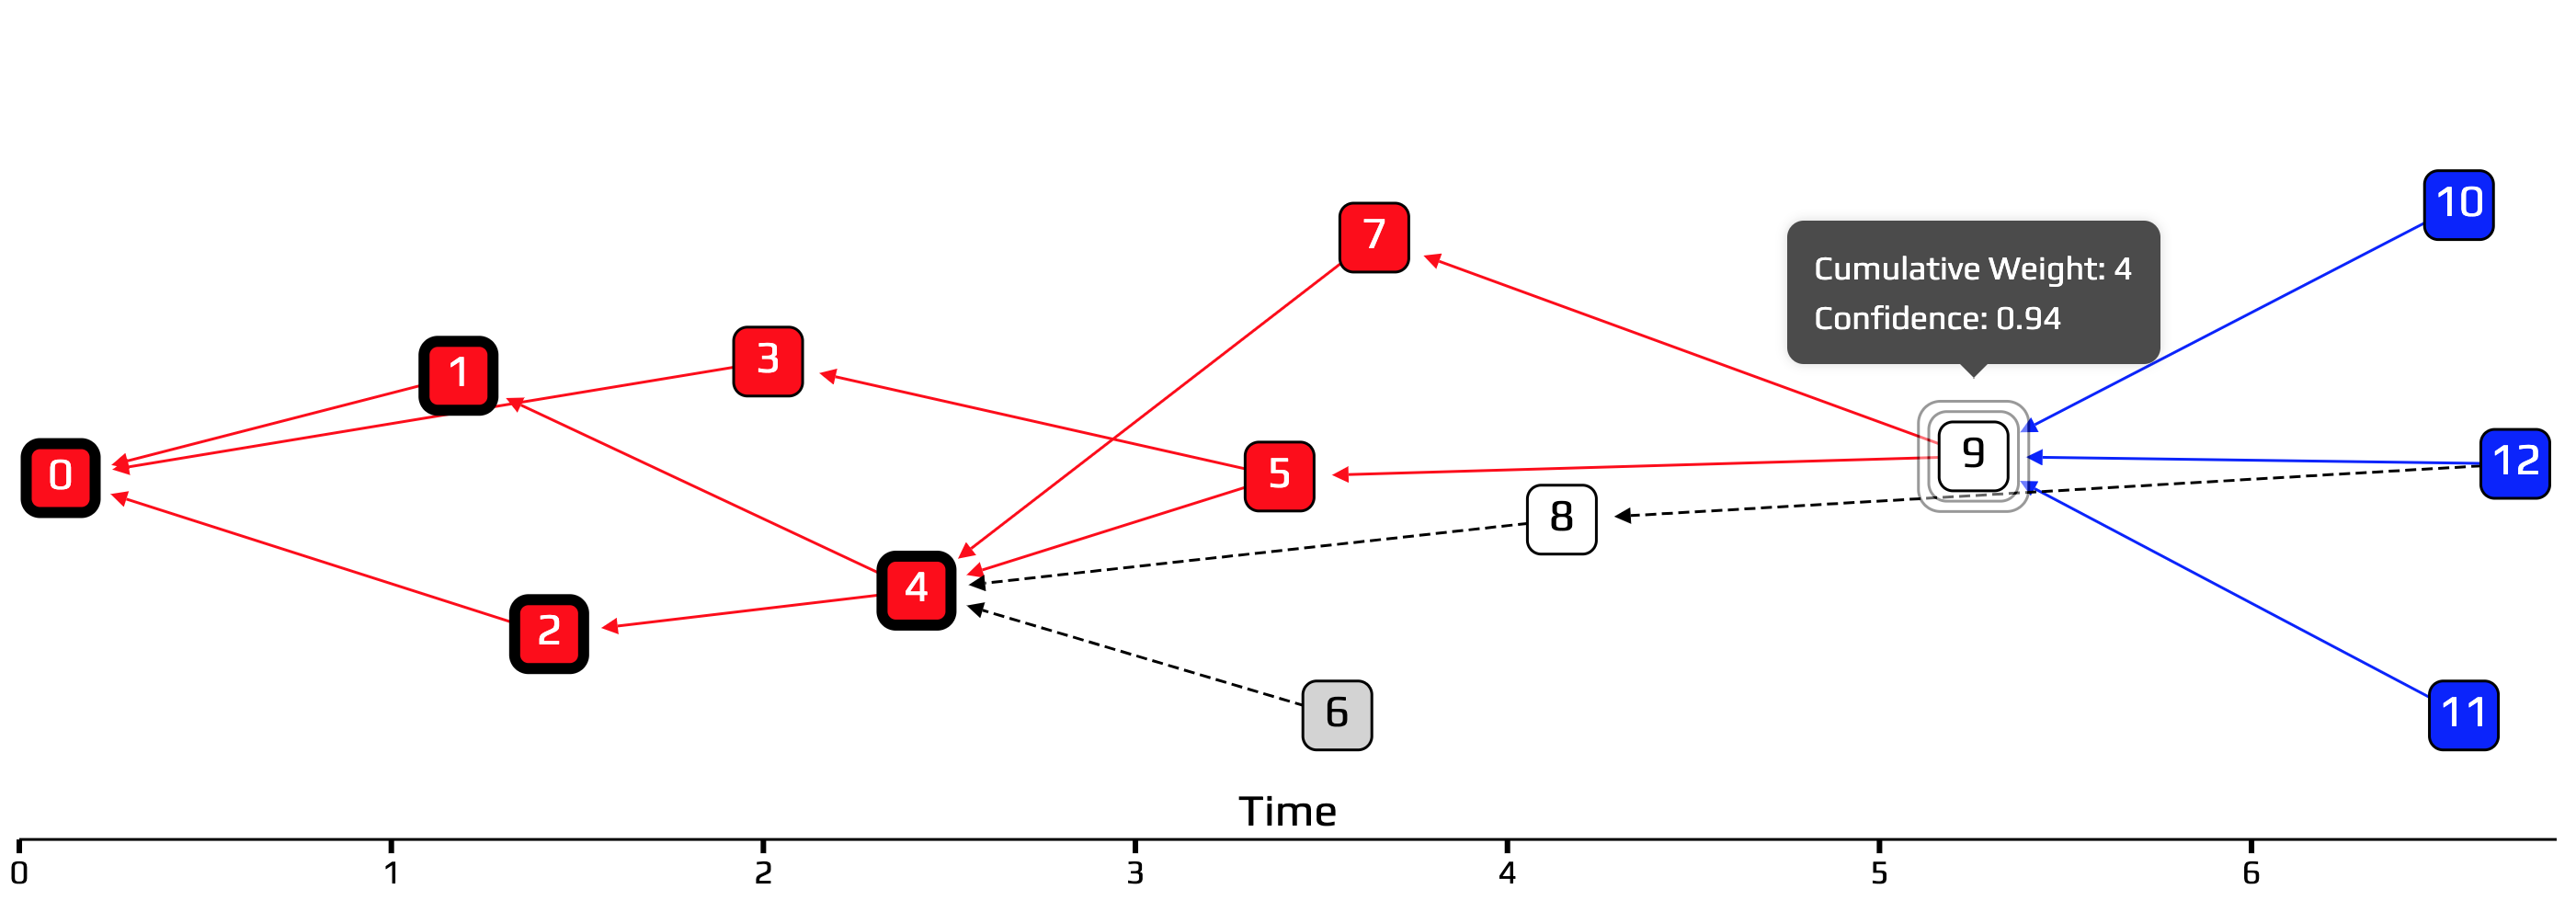
\includegraphics[width=1.0\textwidth]{images/confirmation-confidence-tangle.png}
    \caption{Graph Representation of the Confirmation Confidence}
    \label{fig:confirmation-confidence-tangle}
\end{figure}